\section{Design}
\label{sysdesign:Architecture}
The overall design of the control framework is created with the aim to meet the following set criteria.
\begin{itemize}
\item  The system is required to perform automated vessel platform reconfiguration.
\item  The system needs to perform motion control in a collaborative manner, where multiple robots work together to achieve a single goal. 
\item  The system needs to support both above mentioned behaviors simultaneous.
\end{itemize}
Besides hard constraints, several concepts play a key role for making design decisions. 
\begin{itemize}
	\item The framework should support a large amount of-, or arbitrary  configurations.  This creates adaptiveness to a wide set of tasks for modular vessel platforms, which is a key element supporting commercial competitivity.
	\item  Developed solutions are aimed to be general, such that they are applicable or at least meaningful on other ship-systems, environments and scales of operation. This is considered important to stimulate that knowledge gained from the developed experimental setup benefits future commercial implementation.
	\item Solutions are aimed to be modular, such that subsystems are designed to be conveniently swapped out for another (perhaps improved and better performing) version, easing future improvements and increasing reusability of work.
\end{itemize}

The goal of this design is not to optimize an existing system, but to explore a novel combination of behaviors that is expected to be of interest in the near future. 
The ability of succesful assembly needs to be proved, yet successrate and reconfiguration-speed need only be in reasonable limits and magnitude to reflect commercial implementation. Cooperative motion control needs to show convergence of the system to a desired state while a network of robots operate more effective than the sum of individuals, yet quantitiative motion responses need only be stable and within reasonable timeframe. For quantitative performance evaluations (Chap. \ref{chap:evaluation}), criteria are set representing demands of a logistical usecase, shown in Tab. \ref{tab:KPIS}. 

\begin{table}[]
	\centering
	\begin{tabular}{ll}
		Key performance indicator                 & Criteria           \\ \hline
		Risetime*                                 & $t_r$ \textless{}10s      \\
		Settlingtime*                             & $t_s$ \textless{}40s       \\
		Overshoot*                                & ov\textless{}50\%      \\
		Relative motion between connected modules & $\approx 0$      
	\end{tabular}
	\caption{Performance criteria of the designed system. Risetime, Settlingtime and Overshoot pertain criteria for motion control system evaluation, while relative motion between connected modules indicates assembly success. (* evaluated for step inputs 1.0 \& 0.5m translation and 90grad rotation as characteristic motions)}
	\label{tab:KPIS}
\end{table}

Description on design of the experimental setup starts from a high level view by discussing the multi-robot network topology adapting to varying configurations. It continues to explain the general control approach and division in subsystems that each solve a part of the control problem. Design choices of each subsystem are subsequently discussed in terms of model estimation, state estimation, control effort generation, control effort allocation and  assembly protocol. 

\subsection{Fleet Network Topology}
\label{subsection:topologyDesign}
The modules that are used will be rectangular, equipped with two rotating azimuth thrusters. All modules are identical, so a homogeneous fleet is formed. The design has two axes of symmetry, including weight distribution and thruster placement. The origin of the vessel's body fixed coordinate system will be defined where the planes of symmetry coincide. 
The Reseachlab Autonomous Shipping (RAS) Delft has a fleet of such vessels available, named Delfia's (figure \ref{fig:DelfiaOverallLook}). The vessels dimensions are approximately 380 mm long and 200mm wide. The latest version (the Delfia-1* ) is intended to be equipped with a Raspberry-Pi to perform some on board computation tasks whilst also enabling communication via WiFi. 
\begin{figure}[H]
	\centering
	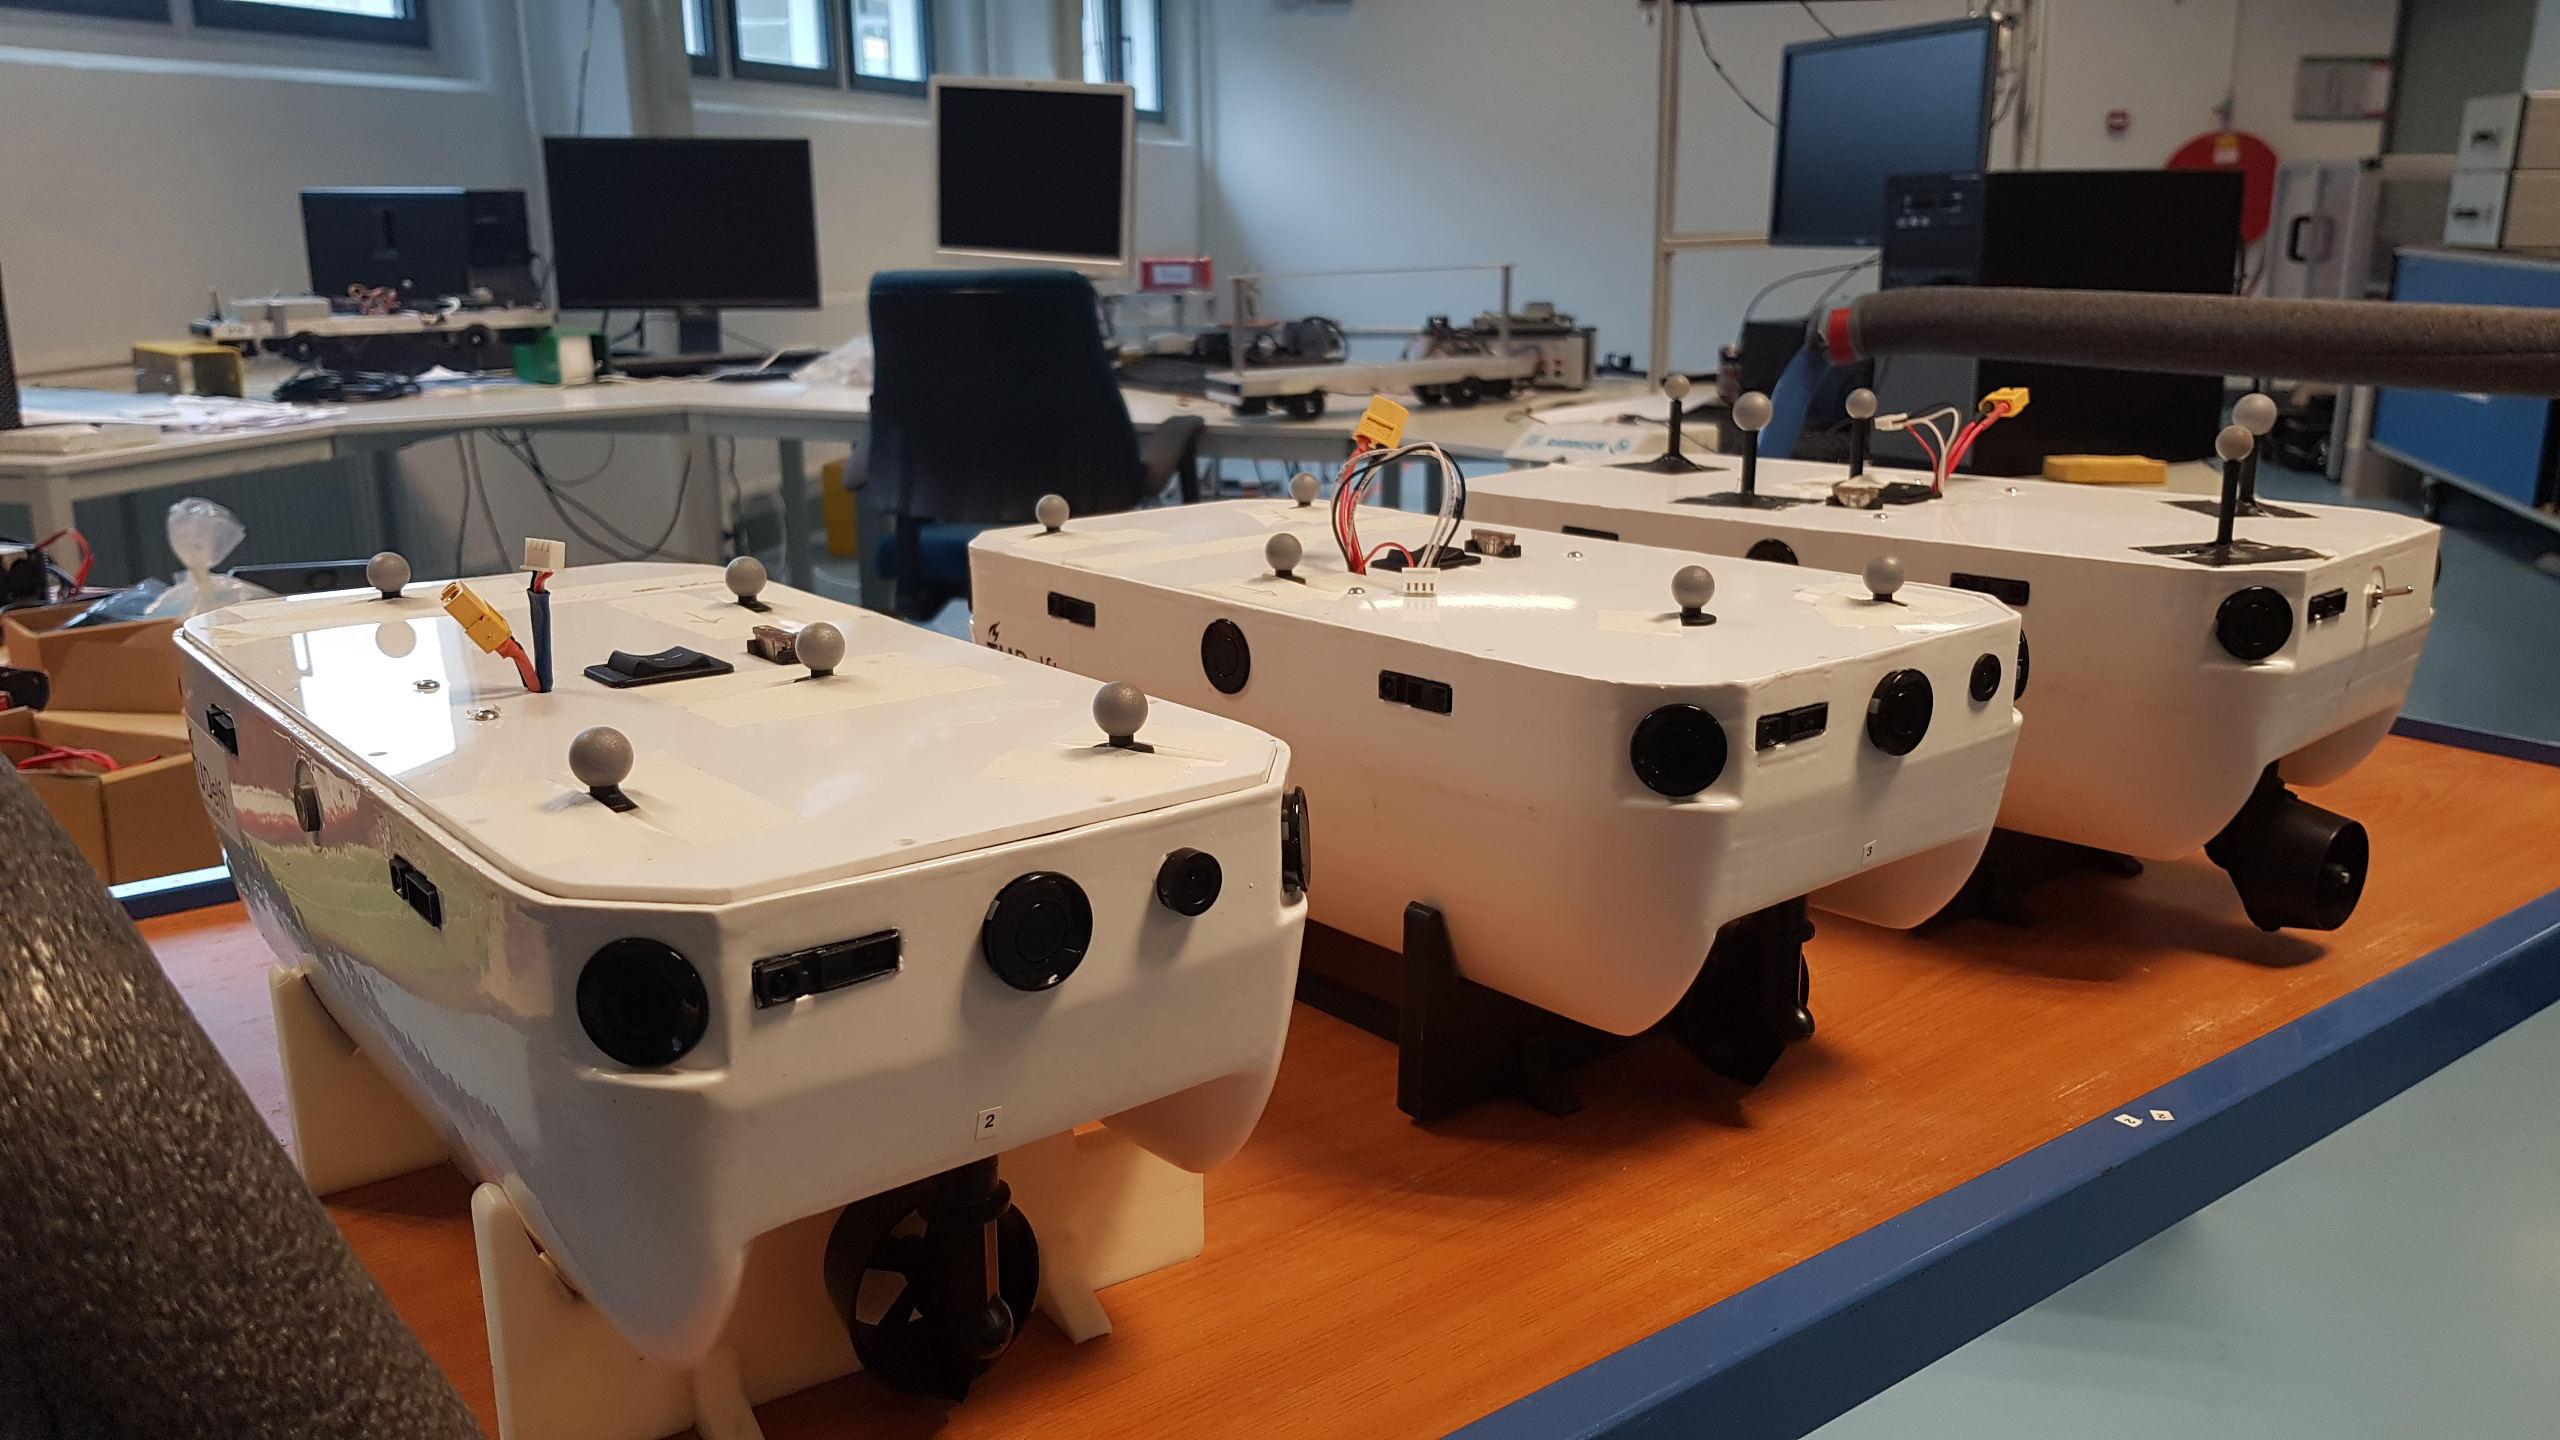
\includegraphics[width=0.9\textwidth]{20210414_121115}
	\caption{Delfia-* vessels, that will act as modules of the fleet system, to perform automated assembly and control.}
	\label{fig:DelfiaOverallLook}
\end{figure}

The approach of dividing a vessel control system via the Guidance, Navigation and Control categorization (\citet{fossen2011handbook} \& section \ref{analysisConfigAdaptation}) is used to distinguish between different system processes. However, the control for this particular system does refer to that of a single vessel, but rather to a set of vessels, which sometimes are controlled individually (when a module moves alone), and in other times together (in assembled platform). Hence, not only the system behavior changes (such as inertia of a platform of variable shape and size), but also the control structure. 


A control structure has been developed, working on three levels, depicted in figure \ref{fig:networkTopology1}. The concept of a 'platform' and a corresponding platform-controller are key to the functioning of this system.  Various tasks of the system are divided across agents that can be roughly described as follows:

\begin{itemize}
	\item A fleet manager
	\item A platform manager
	\item A module
\end{itemize}

\begin{figure}[h]
	\centering
	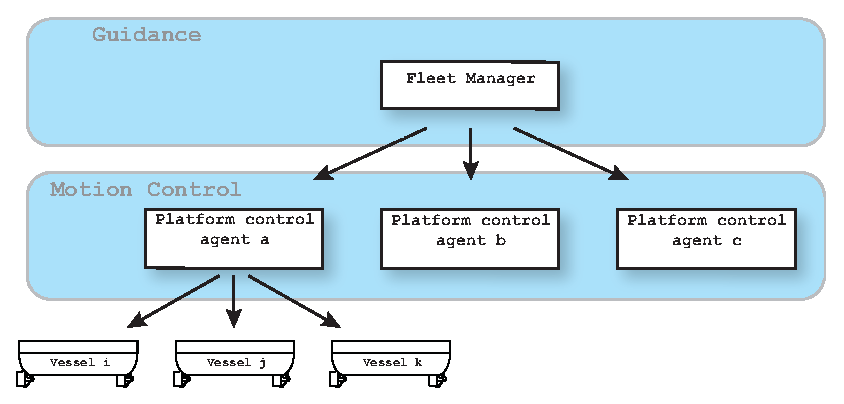
\includegraphics[width=0.9\textwidth]{networkTopology1V2}
	\caption{Hierarchical topology of the network. A single agent manages various platforms control agents. Platform control agents each manage a unique set of modules.}
	\label{fig:networkTopology1}
\end{figure}

A single fleet manager performs vessel guidance and coordination of the assembly process. These tasks are designed to operate as a rather simplistic state machine that runs trough phases based on system triggers or operator input. 

Tasks generated by the fleet manager are passed onto a set of Platform-controllers, which manage motion control of a set of connected modules in a centralized fashion. For every platform, a single agent is responsible for making decisions for all modules in the platform. This platform controller uses a reference state and a platform-state estimation to generate actuator responses for all modules. These are sent to the corresponding modules that make up the platform, which are then interpreted and executed. The platform controlling agent can be embodied by a computer anywhere on the network, given that it has sufficient computational power and the network is stable and reliable. 

The amount of modules that an platform-control-agent manages varies over time as vessels attach or disconnect. Thus all functions of the platform controller needs to be able to handle a variable amount of modules and configured shape. 

Communication between agents is facilitated by WiFi and the Robotic Operating System (ROS) as middleware. ROS facilitates communication between agents in a multi-robot system in an interoperable and modular way. This is thanks to the publisher-subscriber approach, which allows a variable amount of agents to listen (subscribe) to a dedicated datastream (topic). Similarly, a variable amount of agents can send (publish) various datatypes to such topics. This middleware has several benefits, one of which is the ability to set up various topics that represent some system information, on which agents running on various operating systems can send and receive data. The publisher-subscriber approach allows agents to only be subscribed to topics which are relevant. Furthermore, ROS also has many standardized message formats, libraries, and a large and rapidly developing userbase that further enhances interoperability.

State estimation of modules is done by an on-shore optical tracking system. Each vessel has a dedicated topic on which these estimates are published, which are accessible for all entities within the network by subscribing to that particular topic. 

The fleet manager has, besides creating references for the platforms, also the task of coordinating module ownership. As (dis)assembly criteria are met, platform controllers exchange ownership of a module. This informs a platform-controller that a module is connected, and that it now has access to utilizing that module's actuators. Figure \ref{fig:ownershiptransfer1} and \ref{fig:ownershiptransfer1} illustrate transfer of ownership of a module between two platform controllers, which can leave platform-controller-agents without modules under it's control, rendering it inactive. 
Each module will be controlled by a single platform-controller at a time. The platform controller will have full knowledge of the determined pose of each module in the platform with respect to the platform-coordinate system. 

 \begin{figure}[H]
	\centering
	\makebox[\textwidth][c]{
		\begin{minipage}{0.45\textwidth}
			\centering
			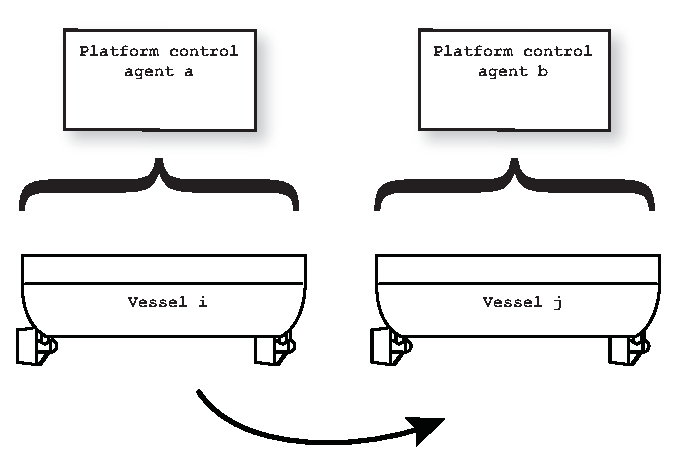
\includegraphics[width=0.95\textwidth]{img/controlAgent_separate}
			\caption{Two vessels that are both controlled by a separate control agent. A change in control structure can transfer module ownership (arrow).}
			\label{fig:ownershiptransfer1}
		\end{minipage}\hfill
		\begin{minipage}{0.45\textwidth}
			\centering
			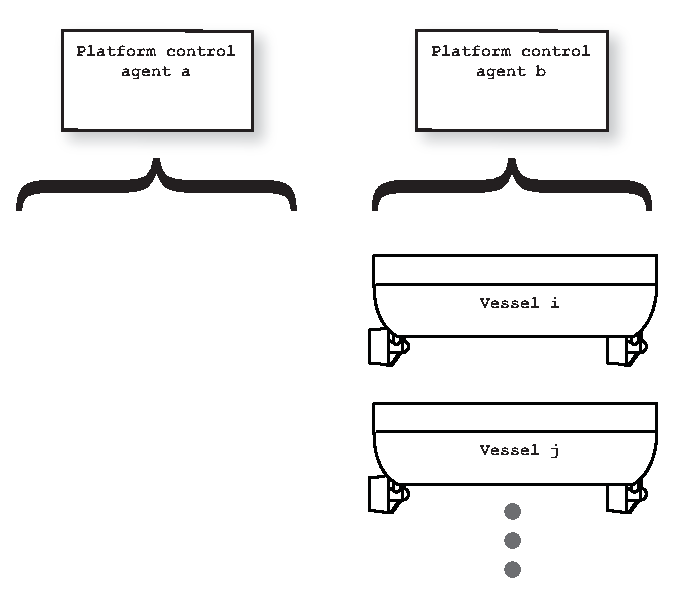
\includegraphics[width=0.95\textwidth]{img/controlAgent_together}
			\caption{Two vessels that formed into a platform, after which they are both controlled by the same agent.}
			\label{fig:ownershiptransfer2}
		\end{minipage}
	}
\end{figure}

\subsection{Platform Level Control Approach}
\label{subsection:PlatformControlApproach}
The platform controller has the goal of generating and publishing actuator commands for connected modules such that the platform motion follows the reference given by the fleet manager. 
The combined structure formed by the assembling modules will have a changing size and shape . This results in variable platform dynamics and number of available actuators. The overall approach on controlling the platform is illustrated in figure \ref{fig:motionControlApproach}. 
As modules connect or disconnect, the platform controller forms a model of the structure in the new configuration. The approach for estimating this model is elaborated in section \ref{platformModel}. Motion control is based on state feedback, where control effort generation and allocation are separated. The control effort generation block uses the estimated model to adapt actuator behavior to maintain performance while the system dynamics change. 
This control approach considers planar motion in 3-DOF (x, y, and yaw), neglecting pitch, heave and roll. 

\begin{figure}[H]
	\centering
	\captionsetup{justification=centering}
	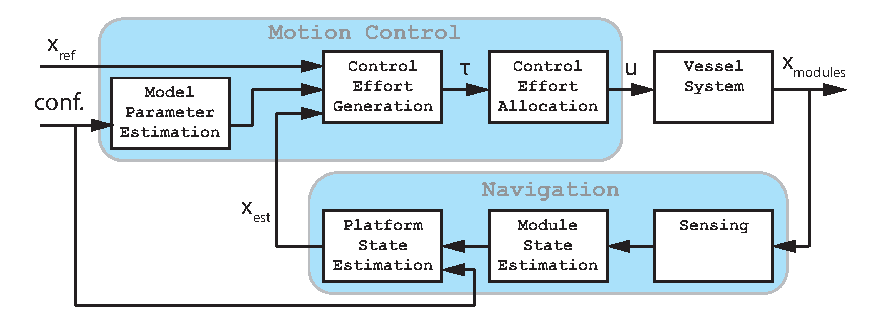
\includegraphics[width=150mm]{MotionControlAndNavigationLoopV3}
	\caption{The designed platform-motion control loop. State reference $X_{ref}$ is the main input from the Fleet manager (guidance system) and output is vessel state $X$. Occasional changes to configuration are communicated to the platform motion controller for adapting control strategy.}
	\label{fig:motionControlApproach}
\end{figure}

The goal is to find actuator commands for all modules under command of the controller such that the platform state approaches a reference state given by the fleet manager. The reference state will be a position and heading, noted as

\begin{equation}
X_{ref} = \eta_{ref} = \begin{bmatrix} x_{ref}\\ y_{ref} \\ \Psi_{ref} \end{bmatrix}
\label{eqPlatformControlRef}
\end{equation}
which is expressed in $\{n\}$. Note that other approaches might also include velocities as a state that is to be controlled, making the reference, estimated and actual state $X$ a [1x6] vector for motion in the surface plane instead of the [1x3] description as shown in equation \ref{eqPlatformControlRef}.

The control problem is solved in the following steps
\begin{itemize}
	\item An approximate model of the combined body is formed. Control gains are adjusted to estimated model parameters. 
	\item Platform state is estimated
	\item From this model, reference state and estimated state - control efforts are generated by means of a proportional-integrator-derivative (PID) controller.
	\item Control efforts are allocated between actuators on the modules. 
\end{itemize}

The state of the platform is defined as the origin and orientation of platform-body-fixed coordinate system $\{p\}$, expressed as 

\begin{equation}
\eta_{p/n}^{n} = \begin{bmatrix} x_{p/n}^{n}\\ y_{p/n}^{n} \\ \Psi_{p/n}^{n} \end{bmatrix}
\end{equation}

which is expressed in $\{n\}$. Note that platform origin is not defined to coincide with the centre of gravity. Connection of a module to the platform is considered binary, meaning a module would be either connected or disconnected, and cannot be 'connected a little'. Any change in platform configuration would result in an instantaneous displacement of the centre of gravity. As continuity of estimated state is desirable, the use of the centre of gravity was avoided to use as the definition of $\{p\}$.




\subsection{State Estimation}
\label{sec:stateEstimationDesign}

%From a set of sensors (on ships or shore) an estimation of the 'platform state' needs to be made. From this, and information of the modules that make up the platform
The platform state is but a concept to represent a collection of modules and is thus not directly measurable. It is however estimated by using a feedback signal of module positions and their known, constant placement within the body. Signal from a separate system performing state estimation of modules is translated to yield platform state estimates. Module localization can be done on board, on shore and with a variety of sensor systems, yet only needs to be consistently communicated on the robot network. Consider an update of the position and orientation of a module as
\begin{equation}
\eta_{b/n}^{n} = \begin{bmatrix} \textbf{p}_{b/n}^{n} \\[10pt] \Psi_{b/n}\end{bmatrix} = \begin{bmatrix} \textbf{x}_{b/n}^{n} \\[10pt] \textbf{y}_{b/n}^{n} \\[10pt] \Psi_{b/n}\end{bmatrix} 
\end{equation}

The known position of modules with respect to platform coordinate system as described by equation \ref{eq:moduleStaticPlacementEtaDefinition} is used to transform module to platform pose by subsequent rotation and translation. For the three considered degrees of surface plane motion the platform state becomes

\begin{equation}
\eta_{p/n}^{n} = \begin{bmatrix} \textbf{p}_{p/n}^{n} \\[10pt] \Psi_{p/n}\end{bmatrix}
\end{equation}
where
\begin{equation}
 \Psi_{p/n} = \Psi_{b/n} - \Psi_{b/p}
\end{equation}
and
\begin{equation}
\textbf{p}_{p/n}^{n} =  \textbf{p}_{b/n}^{n} - \textbf{p}_{b/p}^{n} =  \textbf{p}_{b/n}^{n} - \textbf{R}(\Psi_{p/n}) \textbf{p}_{b/p}^{p} 
\end{equation}


\subsection{Control Effort Generation}
\label{controlEffortGenerationDesign}
The control block is based on a Proportional-Integrator-Differential (PID) controller, designed to scale to model parameters which are estimated as described in section \ref{platformModel}. Three parralel controllers are used to control each individual degree of freedom, as illustrated in \ref{fig:parralelControl1}

\begin{figure}[H]
	\centering
	\captionsetup{justification=centering}
	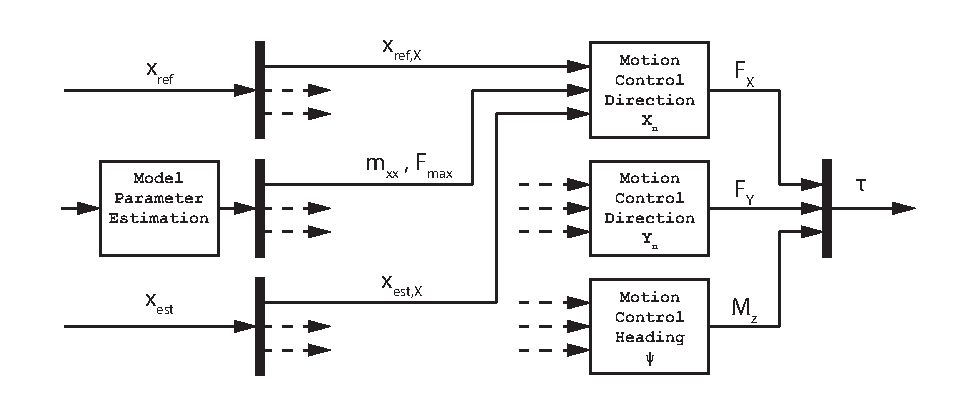
\includegraphics[width=0.9\textwidth]{parralelControl1}
	\caption{Parralel controller setup}
	\label{fig:parralelControl1}
\end{figure}

Control gains of the control-effort-generation block are designed to scale such that, once tuned for a single configuration, show similar behavior for any other configuration or platform size. For this, the following configuration dependent parameters are used. \\

\begin{itemize}
	\item Position of the centre of gravity
	\item Linear inertia, or mass
	\item Angular inertia
	\item Maximum available control effort for translation (maximum force)
	\item Maximum available control effort for rotation (maximum torque)
\end{itemize}

The centre of mass of the platform is found using equation \ref{eq:centreOfMassFindR}. It can then be substituted in equation \ref{eq:translatedToPlatformCentreOfMAss2} to express the equations of motion in that particular point. For three degrees of freedom in the surface plane this becomes shaped as

\begin{equation}
	\textbf{M}_{p}^{CG} = \begin{bmatrix}
	m_{xx} 	&	m_{xy}	& 0 		\\[10pt]
	m_{yx} 	&	m_{yy}	& 0 		\\[10pt]
	0 		&	0		& I_{zz} 	\\[10pt]
	\end{bmatrix}
\end{equation}
where

\begin{table}[H]
	\centering
	\begin{tabular}{ll}
		
		$	\textbf{M}_{11} = \begin{bmatrix}
		m_{xx} 	&	m_{xy}	\\[10pt]
		m_{yx} 	&	m_{yy}	\\[10pt] \end{bmatrix}$ & 
		
		$	\textbf{M}_{12} = \begin{bmatrix}	 0 	\\[10pt]  0	\end{bmatrix}$ \\[25pt]
		
		$	\textbf{M}_{12} = \begin{bmatrix}		0 	& 0 \end{bmatrix}$ &
		
		$	\textbf{M}_{22} =  I_{zz} $
	\end{tabular}
\end{table}



Which shows the estimated moment of inertia $I_{zz}$ in the bottomright corner. If modules have hydrodynamic added mass being modelled as a constant, direction-dependent constant, the off-diagonal elements $m_{xy}$ and $m_{yx}$ may be nonzero. This can also result that masses in $xx$ and $ yy$ direction may be unequal, which can feel rather counter intuitive, as this is never the case with normal rigid body motion. The cause of this still originates from the origonal form of module inertia matrix, as this inherited by using such models. 

The controllers responsible for linear motion will use an estimation of the mass of the platform. Rotating the inertial matrix can be done such that the off diagonal elements $m_{xy}$ and $m_{yx}$ become zero. The magnitude of the diagonal elements can be easily found, as they are the eigenvalues of $M_{11}$. The average of the eigenvalues is used as the estimated omni-directional mass for adapting controller behavior. For linear motion in 2 degrees of freedom (x and y) this becomes
\begin{equation}
	m_{p} \approx \frac{1}{2} \sum_{}^{}  Eig ( \textbf{M}_{11} )
\end{equation}

As the fleet utilizes rotatable azimuth thrusters, the maximum force is generated by the propellers on full power in a single direction. The maximum force that the platform can generate can be found by summation of maximum thruster force of all thrusters
\begin{equation}
\textbf{f}_{p,max} = \sum_{i=1}^{n_{thr}} f_{i,max}
\end{equation}
where $n_{thr}$ refers to the total amount of thrusters, and $f_{i,max}$ is the maximum force that the $i$th propeller can supply. The homogeneous fleet has two identical propellers per module, such that. 
\begin{equation}
\textbf{f}_{p,max} = 2*n* f_{prop,max}
\label{Maxforce1}
\end{equation}

Maximum torque is generated when all thrusters supply maximum force in the direction perpendicular to a vector between CG and the thruster. For a single vessel, this becomes
\begin{equation}
\textbf{m}_{i,max} = |\textbf{r}|  f_{i,max} =  | \textbf{p}_{CG/p}^{p} - \textbf{p}_{thr,i/p}^{p} |  f_{i,max}
\label{maxMoment1}
\end{equation}
where $ \textbf{p}_{CG/p}^{p} $ is the position vector of the platform $CG$ and $ \textbf{p}_{thr,i/p}^{p}$ is the position of the $i$th thruster. The latter is usually given in local frame of a module, but can be converted to platform coordinates by matrix rotation and a translation as:
\begin{equation}
\textbf{p}_{thr,i/p}^{p} =   \textbf{R}_{bj}^{p} \textbf{p}_{thr,i/bj}^{bj} + \textbf{p}_{bj/p}^{p}
\end{equation}
where $\textbf{p}_{thr,i/bj}^{bj}$ is the position of thruster $i$, mounted on module $j$, expressed in the body fixed coordinate system of module $j$. $\textbf{p}_{bj/p}^{p}$ is the position of module $j$ expressed in platform coordinate system. Summation of equation \ref{maxMoment1} over all modules yields total maximum torque generated by actuators for a given configuration as

\begin{equation}
\textbf{m}_{p,max} = \sum_{i=1}^{2n}  \textbf{m}_{i,max}
\label{maxmomentTotalSummed}
\end{equation}

It should be noted that the  equation \ref{Maxforce1} and \ref{maxmomentTotalSummed} show absolute maxima, which need full participation of all actuators to be reached. These maxima can not be obtained in different degrees of motion simultaneously, as outputs will be saturated. To avoid unpredictable control effort generation, actuator operation near output saturation is avoided during implementation.

The control blocks for each degree of freedom, as shown in figure \ref{fig:parralelControl1} operate based on PID control. Generic PID control starts by computing the state error by taking the difference between reference and state feedback. This error is fed parralel trough three different gains, where one signal is integrated and one is differentiated, until the signals are summed to yield the control output.

\begin{figure}[H]
	\centering
	\captionsetup{justification=centering}
	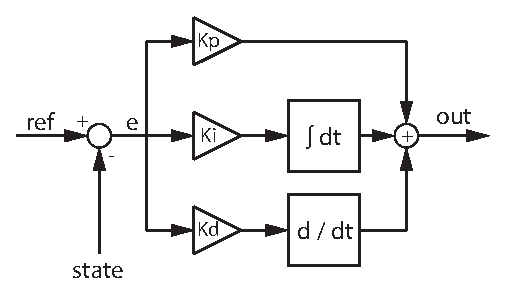
\includegraphics[width=0.4\textwidth]{simplePIDGeneric}
	\caption{A generic Proportional-Integral-Derivative control structure.}
	\label{fig:simplePIDGeneric}
\end{figure}

The control gains of the three parralel PID controllers are tuned to a single reference configuration. As the configuration changes the control gains will adapt to the newly estimated dynamics. 
The control gain scaling is based on the assumption that a configuration will have a response comparable to the reference, but in a different time scale. Typical errors that are fed into PID gains will thus be of comparable magnitude. System responses of current and reference configurations are thus aimed to be approximately comparable such that
\begin{equation}
	\eta_{c}(t) \approx \eta_{ref}(C*t)
	\label{eq:timescaling}
\end{equation}


 If control forces are a dominant factor to the response time of a step input on the system, a characteristic accelleration of a configuration can be defined as
\begin{equation}
a = \frac{Force}{Inertia}
\end{equation}

This is used to estimate the time scaling factor is estimated as the ratio of maximum accelleration of a configuration with respect to the reference configuration. 
\begin{equation}
C_{c} = \frac{a_{c}}{a_{ref}} = \frac{F_{c} \; I_{ref}}{F_{ref} \; I_{c}}
\label{eq:timescaleDef}
\end{equation}
where $ a_{c}$ and $a_{ref}$ are the characteristic accellerations of the current and reference configuration respectively. 

All gains is designed to scale to the maximum obtainable control effort. The base value of contribution is determined in the gain tuning process of the reference configuration. The eventual output of any proportional integral and derivative gains is multiplied by the maximum control effort in that dimention. 

Output of the control effort from proportional gain scales to the magnitude of the error, which assumed comparable in all configurations.  This could result in, for example, a proportional gain that is to contribute 60\% of the maximum obtainable control effort at an error of $e = 1.0$. The gain would become 
\begin{equation}
	K_{p} = K_{p,base}* \tau_{max} =  0.6* \tau_{max}
\end{equation}
such that the control effort contributed by the proportional block becomes
\begin{equation}
	\tau_{i,prop} = e * K_{p} = 0.6* \tau_{max}
\end{equation}

Integral control is however affected by the time in which the system responds. A system that responds slower ( $C_{c} < 1$ ) than the reference configuration will encounter additional integrator buildup. Time factor $C_{c}$ compensates for change of integrator output due to response time by adjusting integral gain as
\begin{equation}
	K_{i} = C_{c} \; K_{p,base} \; \tau_{max}	
\end{equation} 
such that integral control output becomes
\begin{equation}
\tau_{i,int} =  K_{i} \int_{0}^{t} e \; dt =  C_{c} \; K_{p,base} \; \tau_{max} \int_{0}^{t} e dt
\end{equation}

Derivative control output is also affected by time, but scales inversely to time factor $C_{c}$ with respect to integral control. Imagine, for example, a mass (*cough* *cough* vessel) that approaches the reference state, which would make the time derivative of the error negative. Derivative control would attempt to slow the mass down as it approaches it's desired state to avoid overshoot. An object, such as a container vessel, with low maximum control forces relative to the large mass would have to use take this speed more serious than highly manouverable vessels. Derivative adapts to a configuration as
\begin{equation}
K_{i} = \frac{K_{d,base} \; \tau_{max}}{C_{c}}	
\end{equation} 

Base values of controller gains ( $K_{p,base}$ ,$K_{i,base}$ ,$K_{b,base}$ ) will be set while revieuwing responses of the system in reference configuration. A PID controller can be manually tuned, or with the help of many tools such as automated PID tuning software. Linear motion in $x$ and $y$ direction will have identical control settings, as dependency on the orientation of reference frame $\{n\}$ is considered undesirable. 

\subsection{Control Effort Allocation}
\label{controlEffortAllocationDesign}
Control effort, as shown in the previous section, needs to be allocated onto the platform's actuators. The amount of thrusters available varies per configuration. Also placement and orientation of actuators can differ. 
A platform needs to be able to sufficiently control it's motion in all reasonably forseeable configurations. As the amount of different configurations is rather large, a general solution is used, that can solve the control effort allocation problem for all possible configurations. 
The designed control effort allocation protocol relies on the following main principle:
"The contribution of an actuator to a desired resulting force or moment is proportional to   its ability to contribute relative to that of the combined set of actuators."

This principle manifests particularly in rotational motion, as the ability of a thruster to generate torque relies on its placement with respect to the centre of gravity. Linear motion turns out not to exhibit such dependencies, as all thrusters are equal in strength, and possible orientation.  To compute actuator commands that satisfy the desired control effort,
it is allocated in each degree of freedom individually and finally combined.

Position of a thruster with respect to $CG$ can be expressed in $\{p\}$ by
\begin{equation}
\begin{split}
\textbf{p}_{t/CG}^{p} = \textbf{p}_{t/b}^{p} + \textbf{p}_{b/p}^{p} - \textbf{p}_{CG/p}^{p} \\
= \textbf{R}_{b}^{p} \textbf{p}_{t/b}^{p} + \textbf{p}_{b/p}^{p} - \textbf{p}_{CG/p}^{p}
\end{split}
\end{equation}

Thruster force vector can be expressed in $\{p\}$ in 3 degrees of freedom as
\begin{equation}
\begin{split}
\textbf{f}_{t}^{p} = \textbf{R}_{b}^{p} \textbf{f}_{t}^{p}
\end{split}
\end{equation}

The total resultant control effort from all modules in the centre of mass can be found by
\begin{equation}
m_{CG} = \sum_{i =1}^{n_{thrusters}} \textbf{p}_{ti/cg} \times \textbf{f}_{ti}
\label{torqueCG1}
\end{equation}
\begin{equation}
f_{CG} = \sum_{i =1}^{n_{thrusters}}  \textbf{f}_{ti}
\end{equation}
or in vector form as
\begin{equation}
\tau_{CG} = \sum_{i =1}^{n_{thrusters}}  \textbf{H}^{\top}(\textbf{p}_{t/CG}^{p}) \begin{bmatrix}
\textbf{f}_{ti}^{p} \\ 0_{1x3}
\end{bmatrix}
\end{equation}
where $\textbf{p}_{ti/CG}$ is the position of the $i$th thruster with respect to the platform's centre of gravity, and $\textbf{f}_{ti}$ refers to the force vector applied by the $i$th thruster.
Where it should be noticed that the zeros represent torque applied by the propeller, as propellers are modelled as a forcevector applied in a point. A resulting moment can be created due to the fact that thrusters are placed at a distance from $CG$.


The approach on generating control effort that results into torque is as follows. A force at a distance from $CG$ creates a higher resulting torque. The linear relation between torque and distance between applied point and $CG$ can be seen in equation \ref{torqueCG1}. Only considering forces in the $xy$ plane gives
\begin{equation}
	m_{zz} = x_{ti/CG} \; f_{y}  \; -  y_{ti/CG} \; f_{x}
	\label{mzz3dof}
\end{equation}
So at a constant force, the generated moment proportionally increases with distance. For a single direction ($x$ or $y$) this would be shaped as shown in figure \ref{fig:rampThrust}. Thruster contibution to torque that is to be deployed proportional to the effectiveness of the thruster results in a quadratic shape. Figure \ref{fig:paraThrust} shows how the quadratic contribution of a thruster at varying distance

\begin{figure}[H]
	\centering
	\makebox[\textwidth][c]{
		\begin{minipage}{0.45\textwidth}
			\centering
			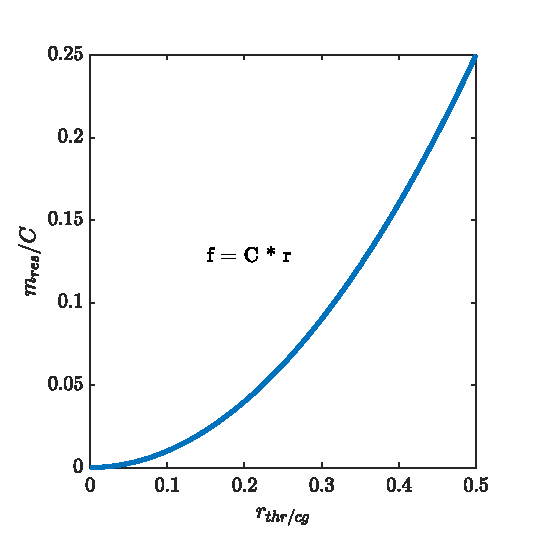
\includegraphics[width=0.95\textwidth]{ThrustAllocPara}
			\caption{Linear relation between resulting moment and thruster distance from $CG$, while thruster force is constant}
			\label{fig:rampThrust}
		\end{minipage}\hfill
		\begin{minipage}{0.45\textwidth}
			\centering
			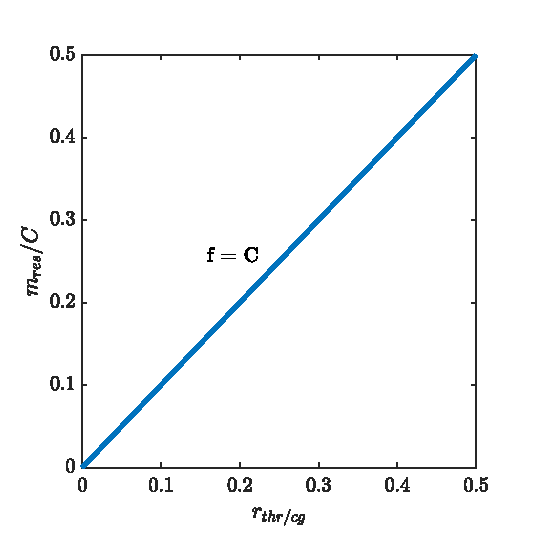
\includegraphics[width=0.95\textwidth]{ThrustAllocLin}
			\caption{Quadratic relation between resulting moment and thruster distance from $CG$, due to a thruster force being controlled to be proportional to distance}
			\label{fig:paraThrust}
		\end{minipage}
	}
\end{figure}

Thruster force to contribute to realizing a desired resulting moment is set as
\begin{equation}
	f_{x} = C_{m} \; m_{d} \; (- y_{ti/CG})
	\label{fx1}
\end{equation}
\begin{equation}
	f_{y} = C_{m} \; m_{d} \; x_{ti/CG}
	\label{fy1}
\end{equation}
where $C_{m}$ is a configuration dependent participation factor for torque and $m_{d}$ is the desired resulting moment of the combined structure. The resulting moment of a thruster becomes (by substituting \ref{fx1} and \ref{fy1} in \ref{mzz3dof})
\begin{equation}
m_{ti} = C_{m} \; m_{d} \; [ x{_{ti/CG}}^{2} \; + \; y{_{ti/CG}}^{2} ]
\end{equation}
The resulting moment of all thrusters satisfies
\begin{equation}
\begin{split}
m_{res} = m_{d} =  \sum_{i =1}^{n_{thrusters}} m_{ti} \\
= C_{m} \; m_{d} \; \sum_{i =1}^{n_{thrusters}}  \; [ x{_{ti/CG}}^{2} \; + \; y{_{ti/CG}}^{2} ]
\end{split}
\end{equation}
From which the total configuration dependent participation factor can be found, as
\begin{equation}
\begin{split}
C_{m} = \frac{1}{ \sum_{i =1}^{n_{thrusters}}  \; [ x{_{ti/CG}}^{2} \; + \; y{_{ti/CG}}^{2} ] }
\end{split}
\end{equation}
This constant ends up scaling all thruster contribution such that the overall relationship between thruster contribution and distance is quadratic, and that the resultant moment matches the desired moment. 


For linear motion a similar principle of contribution to effectiveness is applied, yet turns out much simpler. The homogeneous fleet has thrusters that are all equal in strength, and able to turn in all directions. As all thrusters are thus equally able to contribute to linear motion, total desired thrust is equally divided between all thrusters such that

\begin{equation}
f_{d} = \sum_{i=1}^{n_{thrusters}} * f_{ti}
\end{equation}

\begin{equation}
f_{ti} = C_{f} \; f_{d}\;  f_{max}
\end{equation}

\begin{equation}
C_{f} = \frac{1}{n_{thrusters}}
\end{equation}


All degrees of freedom that are affected by elements from the vector of desired control effort are evaluated independently, resulting in a forcevector for every thruster for every degree of freedom. The forcevectors pertaining to a thruster in all degrees of freedom are summed to obtain the overall contribution of that thruster. For three degrees of freedom this becomes
\begin{equation}
	\textbf{f}_{ti} = \textbf{f}_{ti,fx} + \textbf{f}_{ti,fy} + \textbf{f}_{ti,m}
\end{equation}
Fig. \ref{fig:controlAllocationSeparate1} illustrates how the control allocation problem is solved by combining actuator responses from elements of the desired control effort vector. 

\begin{figure}[H]
\centering
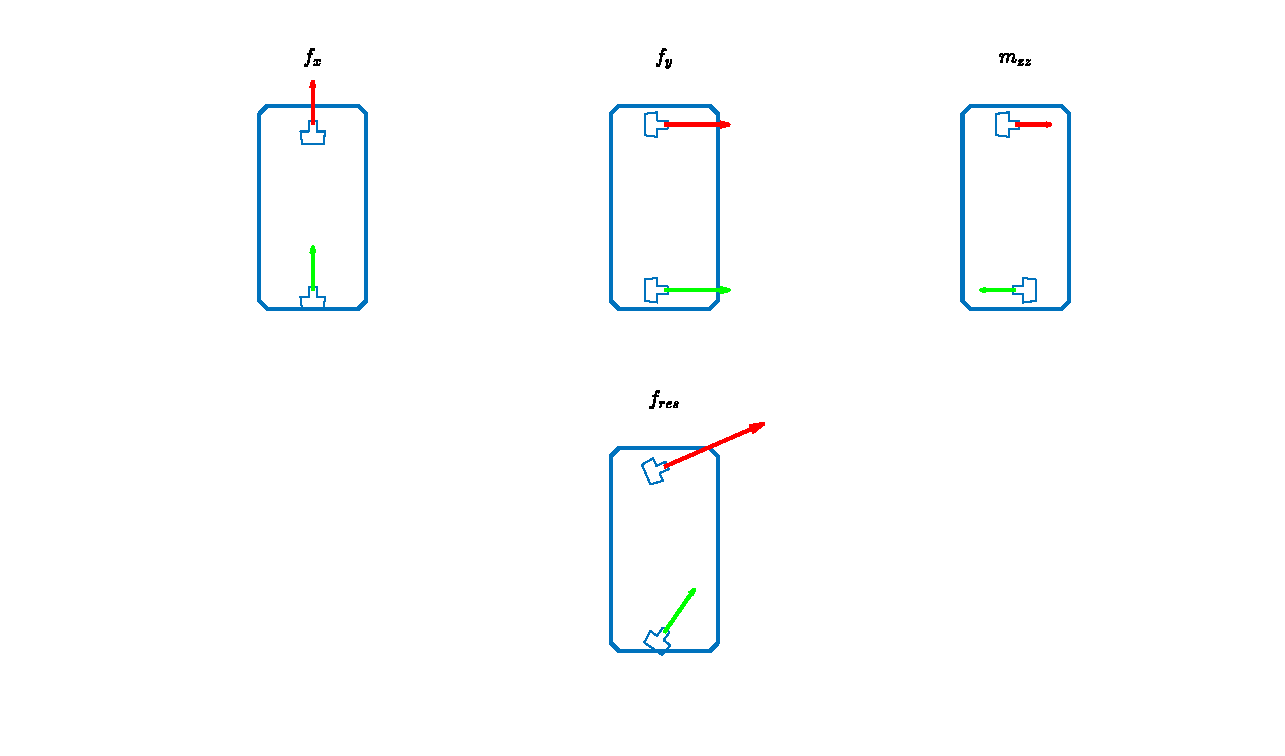
\includegraphics[width=\textwidth]{actuation_combined}
\caption{The approach of solving control allocation in each dimention separately, illustrated for a single vessel configuration. Three dimensions along which control effort is required are solved (above). The forces of the three solutions are combined to yield the final solution (below). }
\label{fig:controlAllocationSeparate1}
\end{figure}

\subsection{Assembly Protocol}
\label{assemblyProtocolDesign}
Modules will assemble in a lattice structure, using active magnets to remain configured. Task execution, including assembly, operates in a phasewise fashion. Generating the desired configuration (blueprint) and assembly planning are done by the operator for this project. 
The following steps are considered to achieve assembly of a module or platform to another:
\begin{itemize}
	\item The connecting object lines up with the assembly at a short distance, such that it can freely reach the connection site. During this process both objects are controlled by different controllers. 
	\item The connecting object moves to the connection site. Magnet connectors within area of acceptance of a connection site make contact, and connect. 
	\item Success of connectivity is evaluated before continuing
	\item If connected, ownership of the connecting bodies is transferred to the controller of the assembly. The other controller becomes inactive. (see figure \ref{fig:ownershiptransfer1} and \ref{fig:ownershiptransfer2})
	\item The controller of the assembly recomputes configuration dependent parameters on:
	\begin{itemize}
		\item The estimated platform model, as in section \ref{platformModel}
		\item The control effort generation protocol, by adapting controller gains to the newfound model estimate, as in section \ref{controlEffortGenerationDesign}
		\item   The control allocation protocol, to divide generated control effort over the new configuration as described in section \ref{controlEffortAllocationDesign}.
	\end{itemize}
	\item The assembly runs the adapted control scheme for further tasks.
\end{itemize}


\begin{figure}[H]
	\centering
	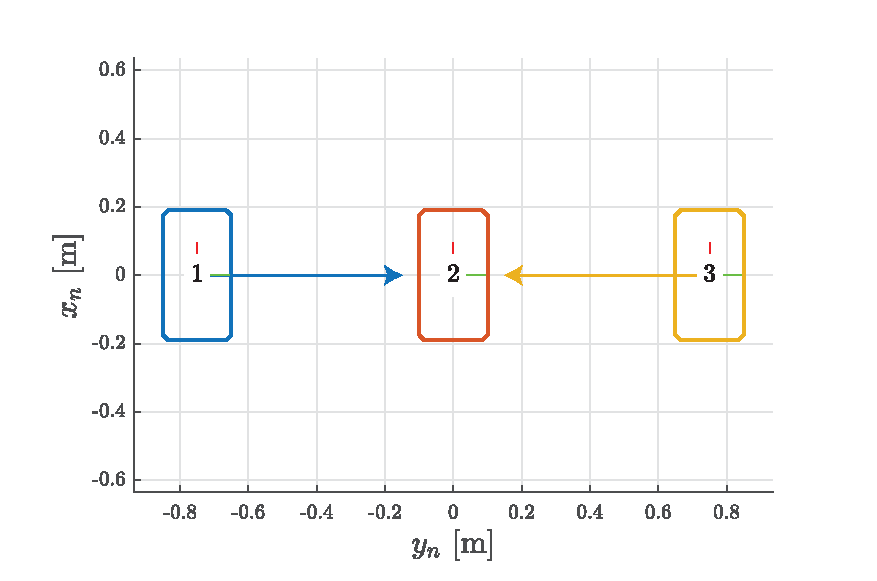
\includegraphics[width=0.7\textwidth]{matlabEvaluationFig14c}
	\caption{Platform assembly protocol from top vieuw. Vessel 1 and 3 are lined up to approach connecting to vessel 2 on either side. Once connectors are within range, the magnets snap into place, fixing relative motion.}
	\label{fig:matlabEvaluationFig14c}
\end{figure}


% The forces and moments represented by the acceleration hydrodynamic coefficients can, to a very great extent, be modeled as potential flow phenomena. Neglecting the details of the boundary layer in modeling acceleration-dependent forces and moments acting on a submerged body yields quite satisfactory results for most stability and control simulation. " \ref{humphreys1978prediction}


	